\chapter{Simple Snake - Klassediagrammer}


\begin{figure}[h]
	\centering
    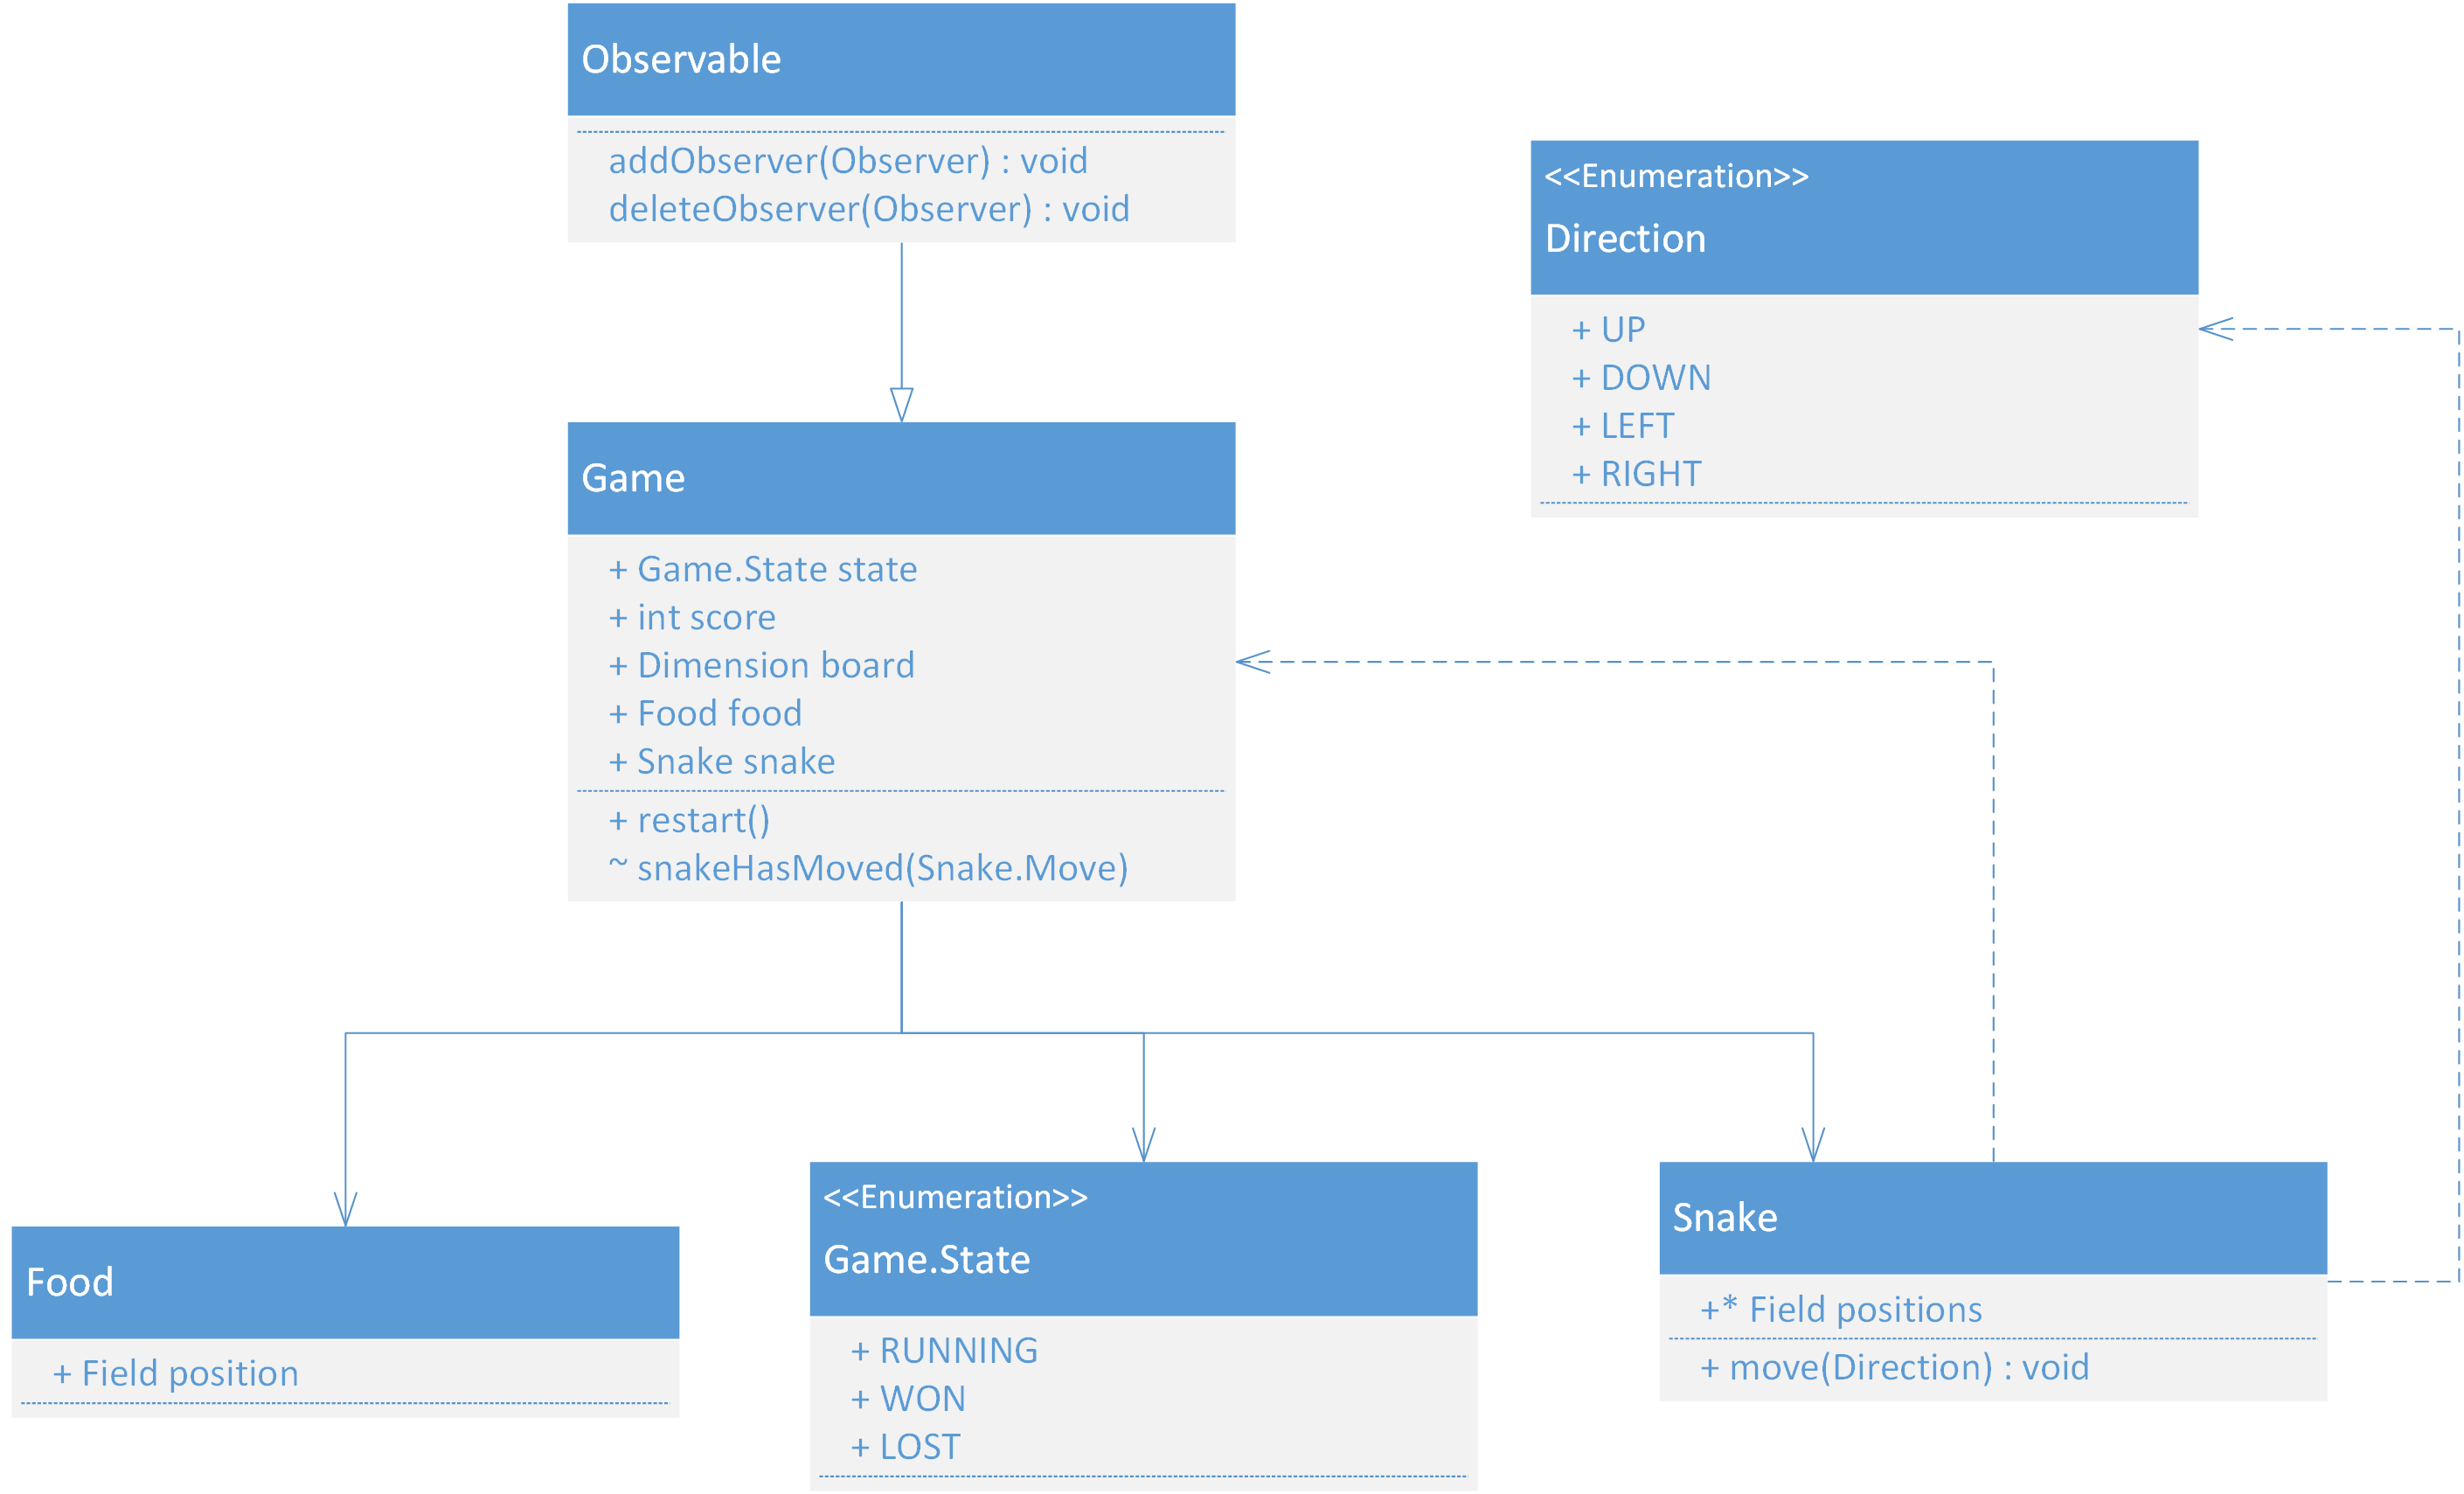
\includegraphics[width=1.0\textwidth]{grundlaeggende/model.png}
	\hspace{0.1\textwidth}
	\caption{\textit{UML klassediagram over Model-pakken.}}
\end{figure}

\begin{figure}[h]
	\centering
    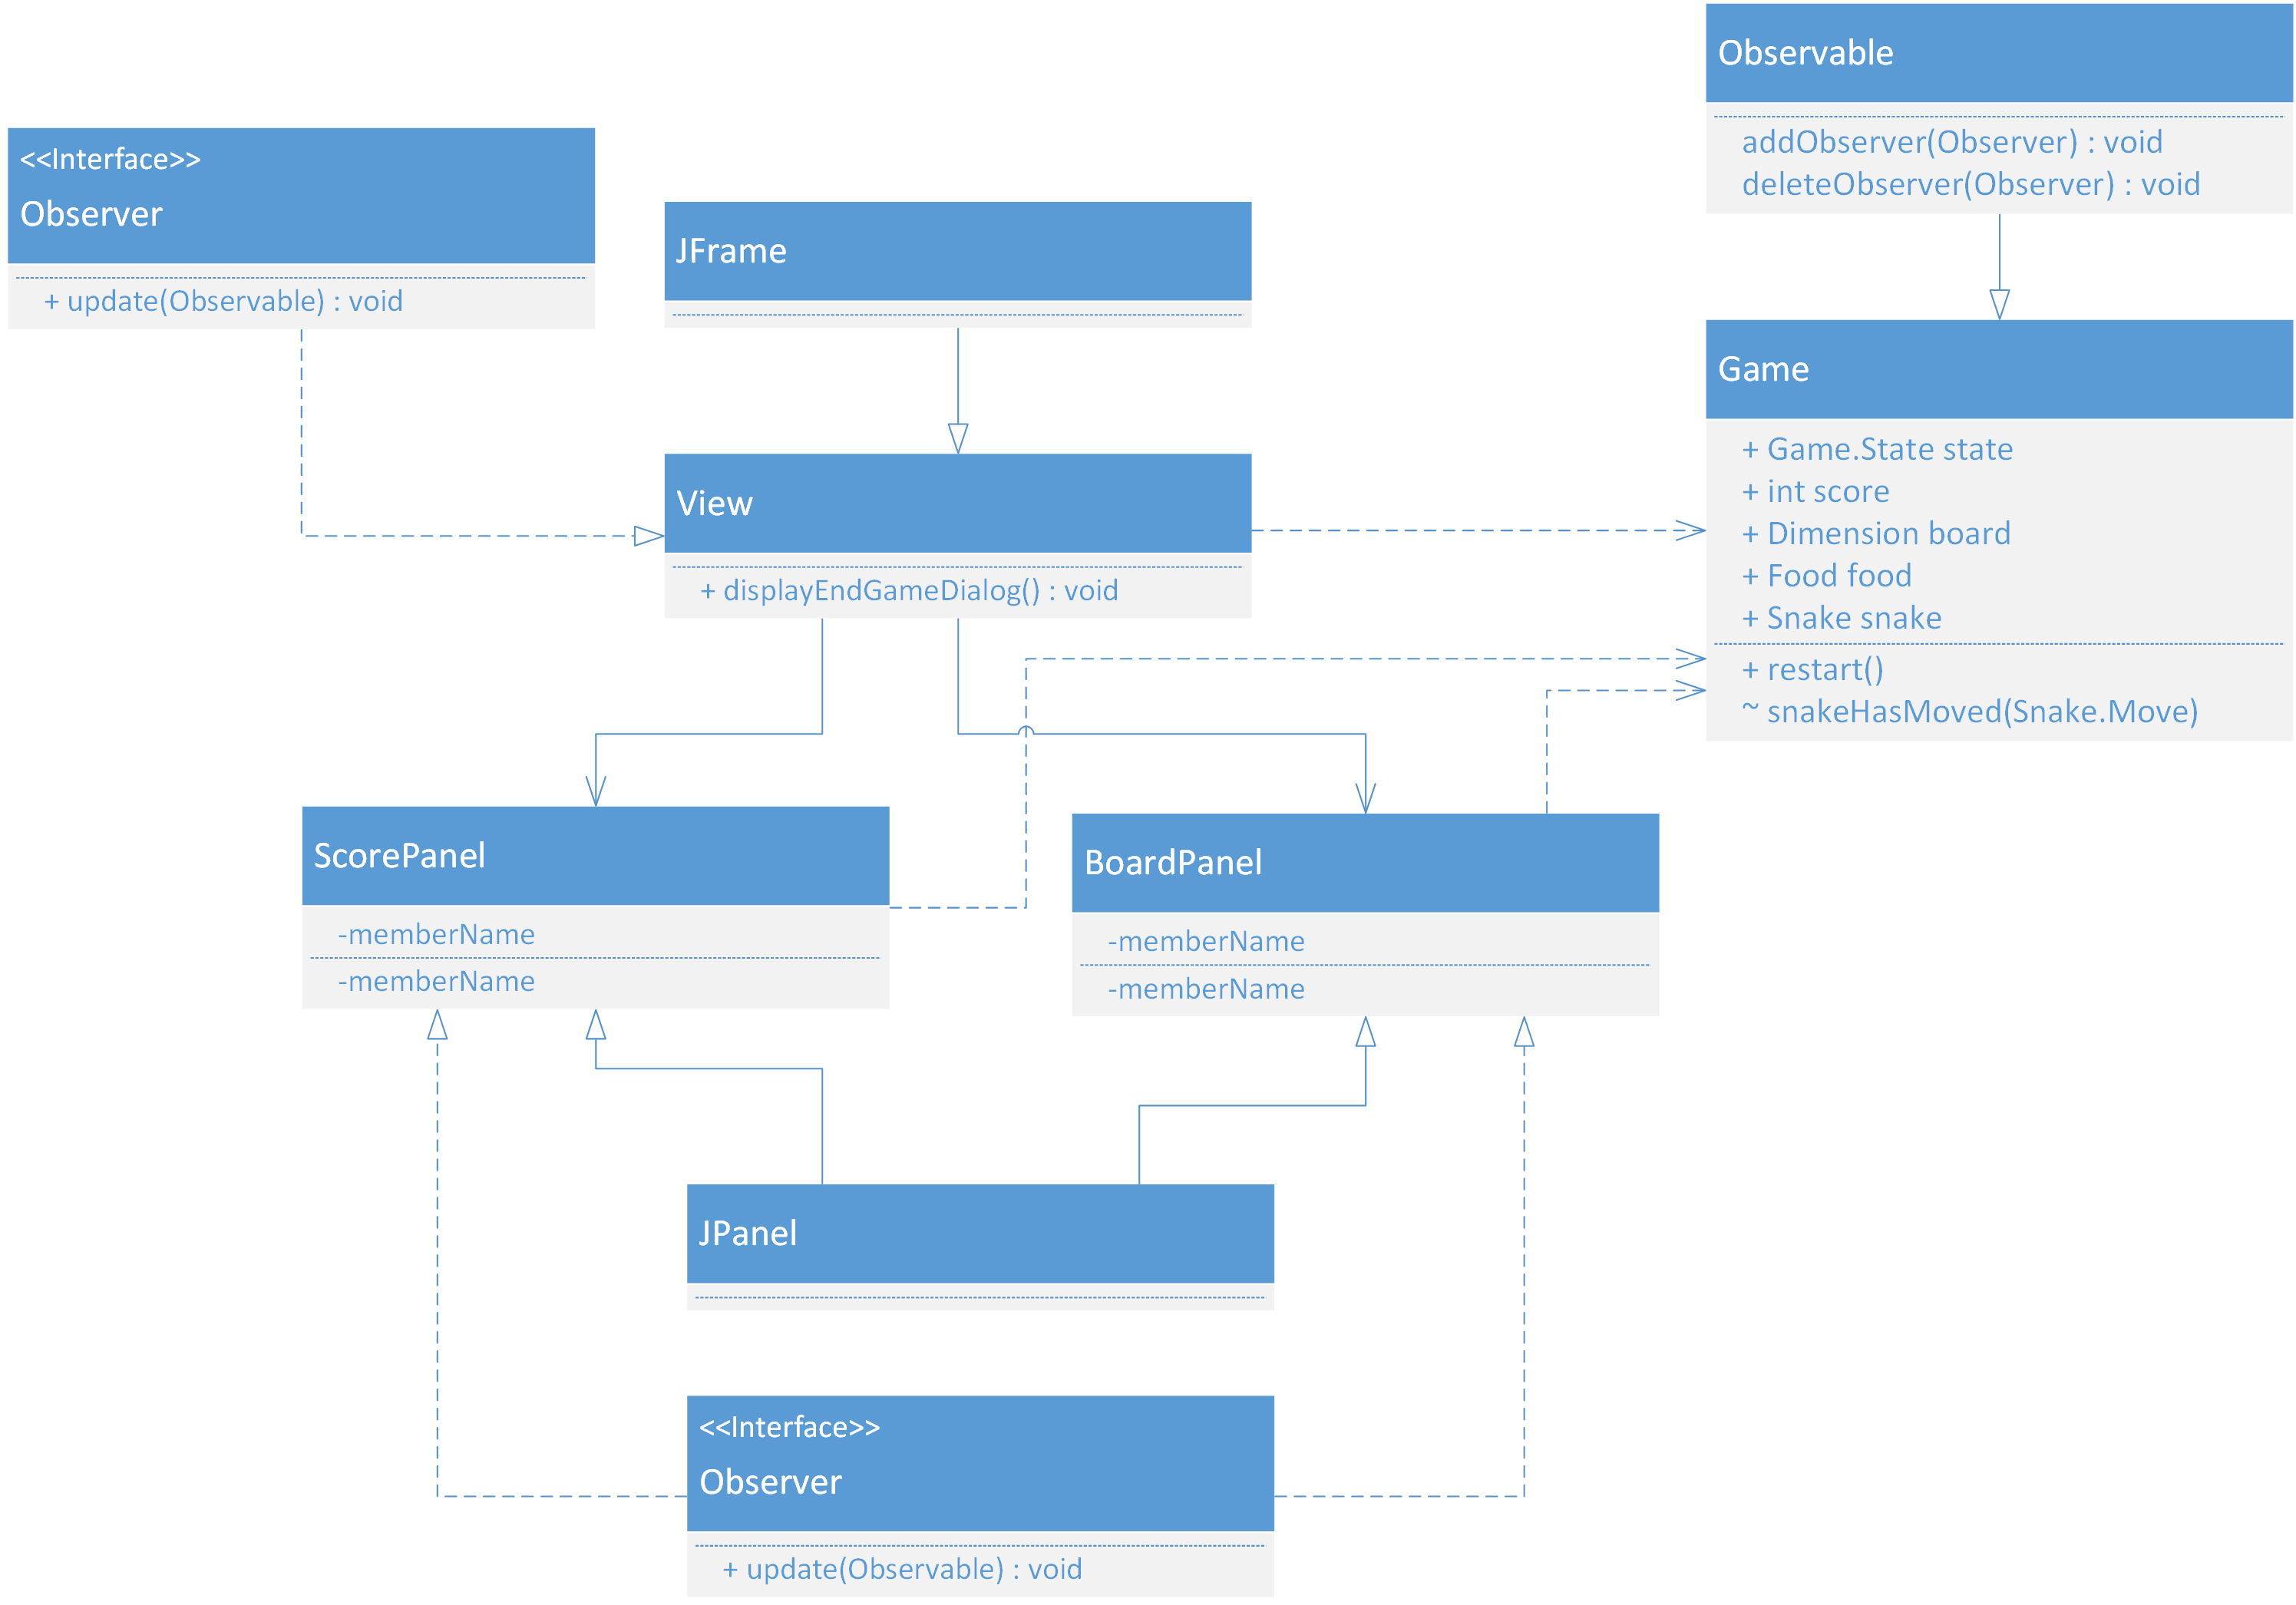
\includegraphics[width=1.0\textwidth]{grundlaeggende/view.png}
	\hspace{0.1\textwidth}
	\caption{\textit{UML klassediagram over View-pakken.}}
\end{figure}

\begin{figure}[h]
	\centering
    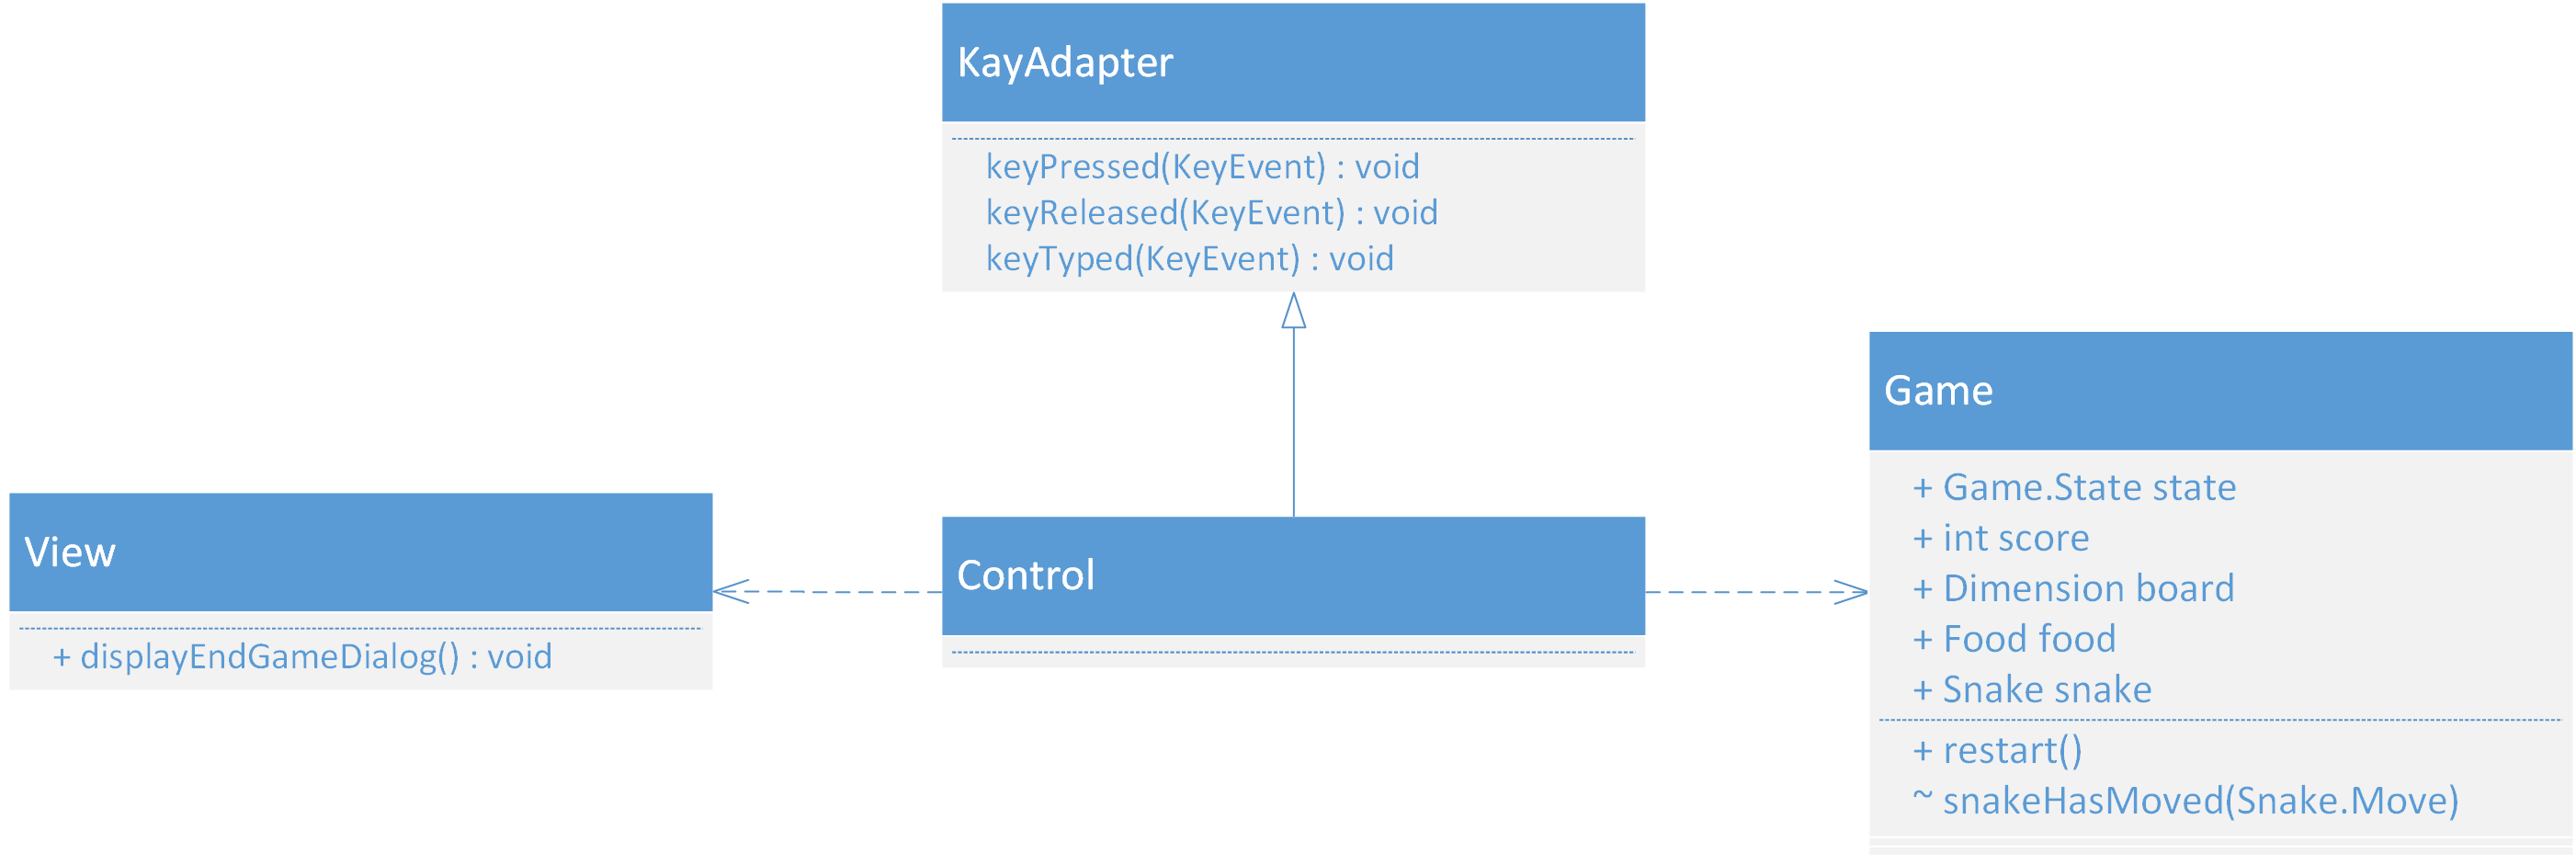
\includegraphics[width=1.0\textwidth]{grundlaeggende/control.png}
	\hspace{0.1\textwidth}
	\caption{\textit{UML klassediagram over Control-pakken.}}
\end{figure}


\chapter{Advanced Snake - Relationsklasser}
\newpage
\begin{center}
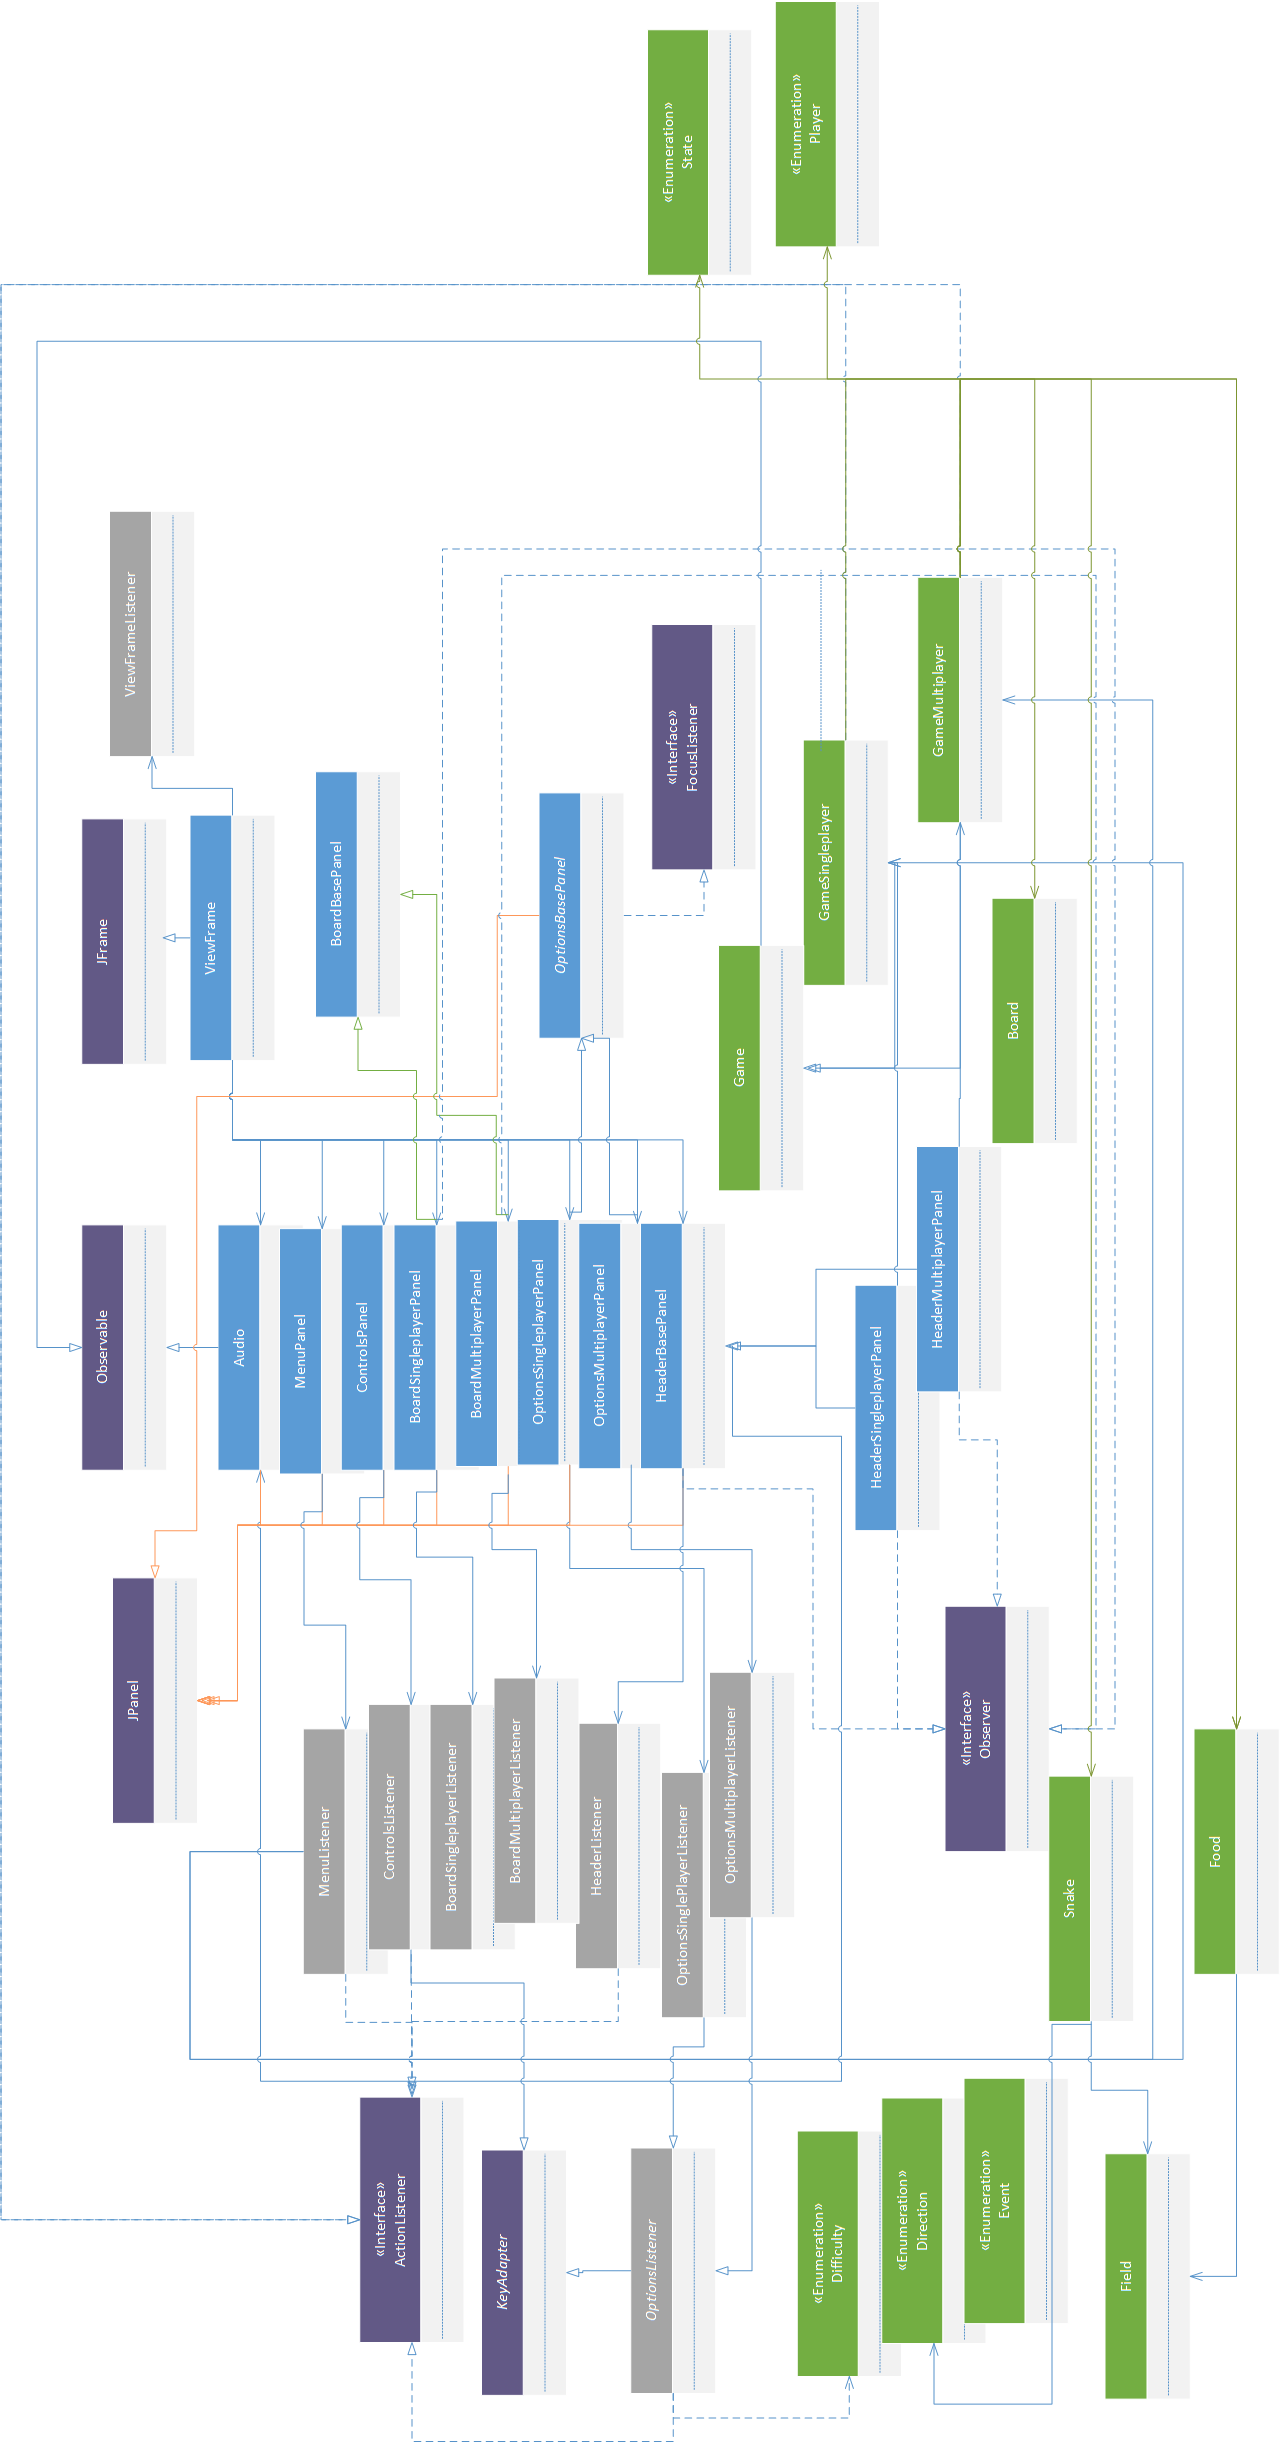
\includegraphics[width=\textwidth,height=\textheight,keepaspectratio]{AdvancedSnakeKlassediagram.png}
\end{center}


\chapter{Slangens opbygning}
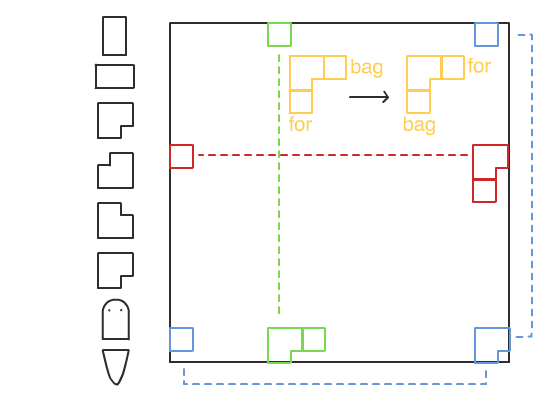
\includegraphics[width=1\textwidth]{SnakeGraphic.png}